\documentclass{article}
\usepackage{listings}
\usepackage{xcolor}
\usepackage{graphicx}


\title{ACN LAB - 03 \\Introduction to Basic Network Commands}
\author{Chaitanya Talware (MIS No: 712422005) \\ Yogesh Toshniwal (MIS No: 712422021)}

\date{}

\lstdefinestyle{python}{
    language=Python,
    basicstyle=\ttfamily\small,
    numbers=left,
    numberstyle=\tiny\color{gray},
    stepnumber=1,
    numbersep=5pt,
    backgroundcolor=\color{lightgray},
    showstringspaces=false,
    frame=single,
    rulecolor=\color{black},
    breaklines=true,
    breakatwhitespace=true,
    keywordstyle=\color{blue}\bfseries,
    commentstyle=\color{green},
    stringstyle=\color{red},
}

\begin{document}


\maketitle
\clearpage  % Ensures the next content starts on a new page
\section{Introduction to Basic Network Commands}
Networking commands are fundamental tools for diagnosing and maintaining computer networks. 
They allow users to monitor network configurations, check connectivity, and troubleshoot potential issues. 
Whether managing a small home network or administering a complex enterprise system, understanding these commands is essential.

This assignment aims to explore widely used network commands such as \texttt{ipconfig}, \texttt{ping}, \texttt{traceroute}, and others, emphasizing their significance in practical scenarios. Each command is detailed with its available options and expected output to provide a clear and comprehensive understanding.

\section{Commands Overview}

\subsection{\texttt{ipconfig}}
The \texttt{ipconfig} command is used to display and manage the IP address configuration of a system. It provides detailed information about network adapters, including their IP addresses, subnet masks, and gateways. This command is commonly used for troubleshooting network issues or updating DHCP settings.

\subsubsection{Options}
\begin{itemize}
    \item \texttt{/?} - Shows a help message with a list of available options.
    \item \texttt{/all} - Displays detailed information about all network adapters.
    \item \texttt{/release} - Releases the IPv4 address for the specified adapter.
    \item \texttt{/release6} - Releases the IPv6 address for the specified adapter.
    \item \texttt{/renew} - Renews the IPv4 address for the specified adapter.
    \item \texttt{/renew6} - Renews the IPv6 address for the specified adapter.
    \item \texttt{/flushdns} - Clears the DNS resolver cache.
    \item \texttt{/registerdns} - Refreshes DHCP leases and re-registers DNS names.
    \item \texttt{/displaydns} - Displays the contents of the DNS resolver cache.
    \item \texttt{/showclassid} - Lists all DHCP class IDs available for the adapter.
    \item \texttt{/setclassid} - Updates the DHCP class ID for the adapter.
    \item \texttt{/showclassid6} - Lists all IPv6 DHCP class IDs available for the adapter.
    \item \texttt{/setclassid6} - Updates the IPv6 DHCP class ID for the adapter.
\end{itemize}

\subsubsection{Example 1}
To view the complete network configuration of all adapters:
\begin{verbatim}
ipconfig /all
\end{verbatim}
\subsubsection{Example 2}

\begin{verbatim}
ipconfig 
\end{verbatim}

% \subsubsection{Command Information and Options}
% Add content here.
Running the \texttt{ipconfig} command without any options provides a concise summary of the network adapter configurations. The output typically includes the following information:

IPv4 Address: The IP address currently assigned to the system.
Subnet Mask: Specifies the size of the network segment.
Default Gateway: The router's IP address used to access external networks.
Connection Status: Indicates whether the adapter is active or disconnected.
\subsubsection{Command Output}

\begin{figure}[htbp]
    \centering
    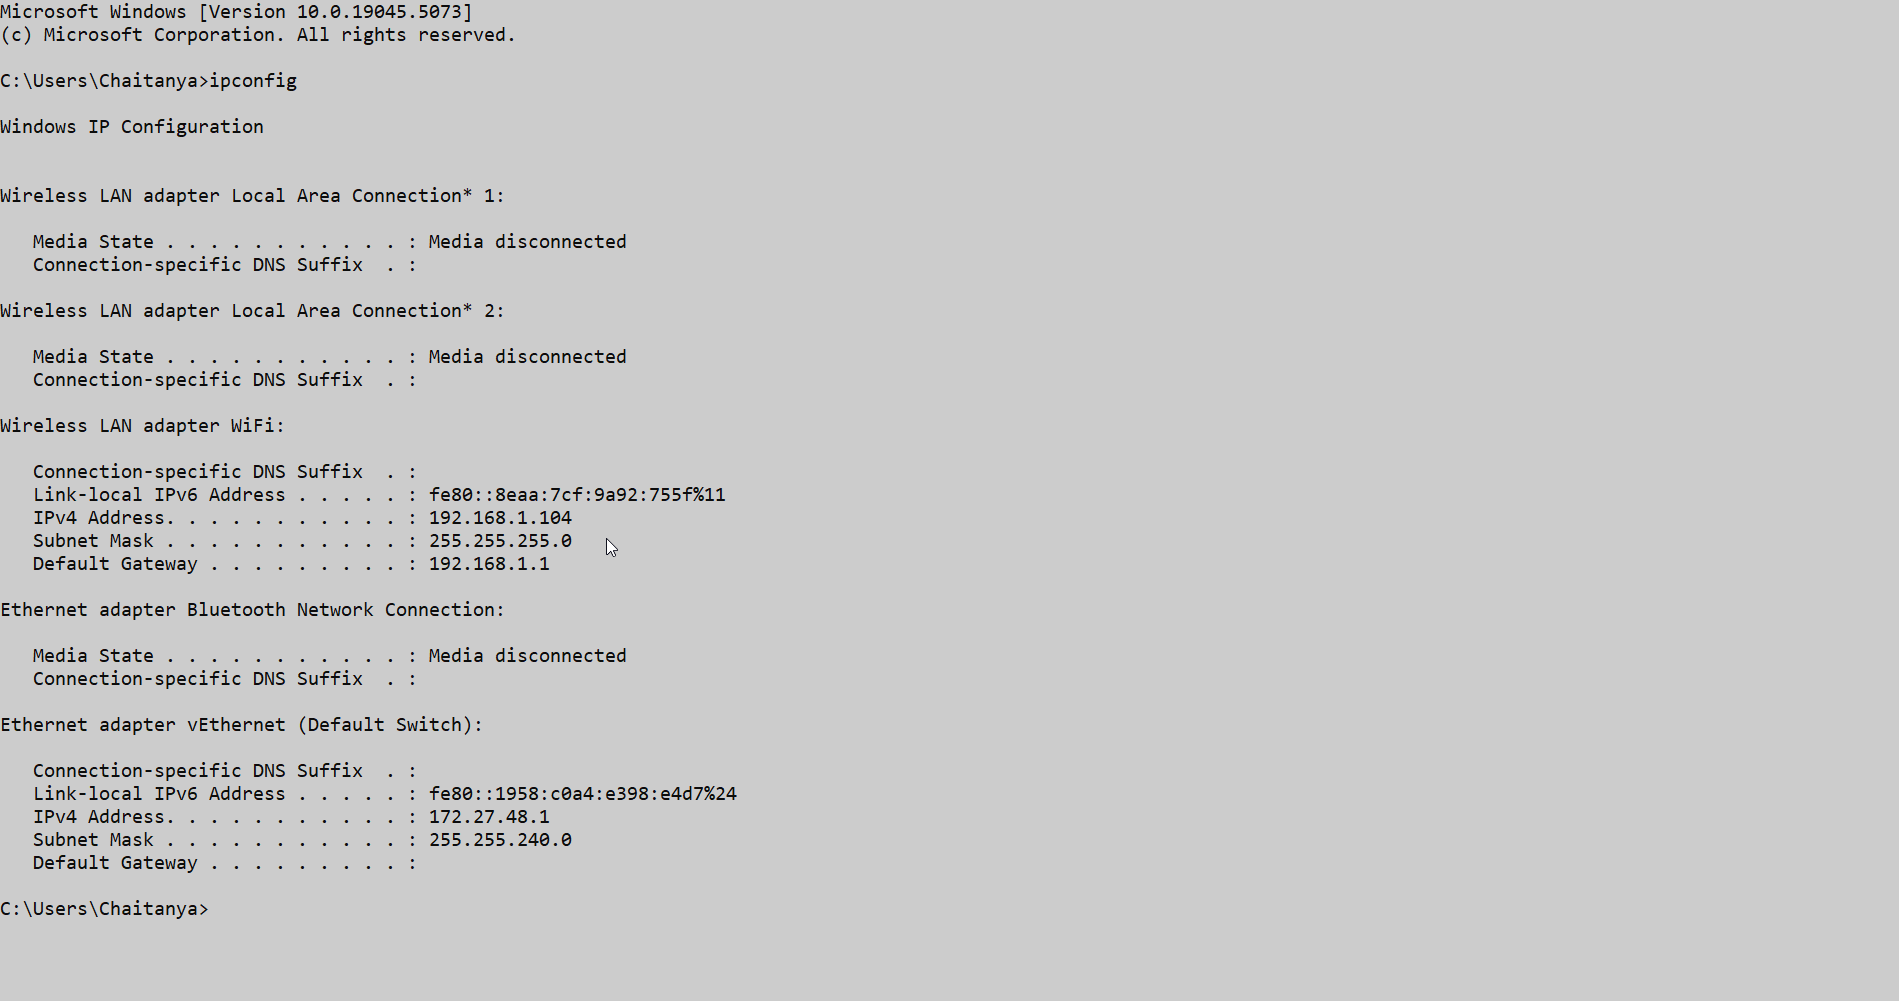
\includegraphics[]{IPconfig.png}
    \caption{ipconfig Command Output}
    \label{fig:ipconfig_output}
\end{figure}


\clearpage % Ensures the next content starts on a new page
\subsection{\texttt{ping}}
The \texttt{ping} command is used to test the reachability of a network host and measure the round-trip time for messages sent from the originating host to a destination. It helps in diagnosing network connectivity issues.

\subsubsection{Options}
\begin{itemize}
    \item \texttt{-t} - Pings the specified host continuously until stopped manually.
    \item \texttt{-a} - Resolves addresses to hostnames during the ping.
    \item \texttt{-n \textless count\textgreater} - Specifies the number of echo requests to send.
    \item \texttt{-l \textless size\textgreater} - Sends packets of a specified size.
    \item \texttt{-w \textless timeout\textgreater} - Sets the timeout (in milliseconds) for each reply.
    \item \texttt{-4} - Forces the use of IPv4 for the ping.
    \item \texttt{-6} - Forces the use of IPv6 for the ping.
    \item \texttt{-f} - Sets the "Don't Fragment" flag in the packet header.
    \item \texttt{-i \textless TTL\textgreater} - Specifies the Time to Live (TTL) value for packets.
    \item \texttt{-r \textless count\textgreater} - Records the route for a specified number of hops.
\end{itemize}

\subsubsection{Example 1}
To send 4 ping requests to the specified host:
\begin{verbatim}
ping google.com
\end{verbatim}

% \subsubsection{Command Information and Options}
% Add content here.


\subsubsection{Command Output}
\begin{figure}[htbp]
    \centering
    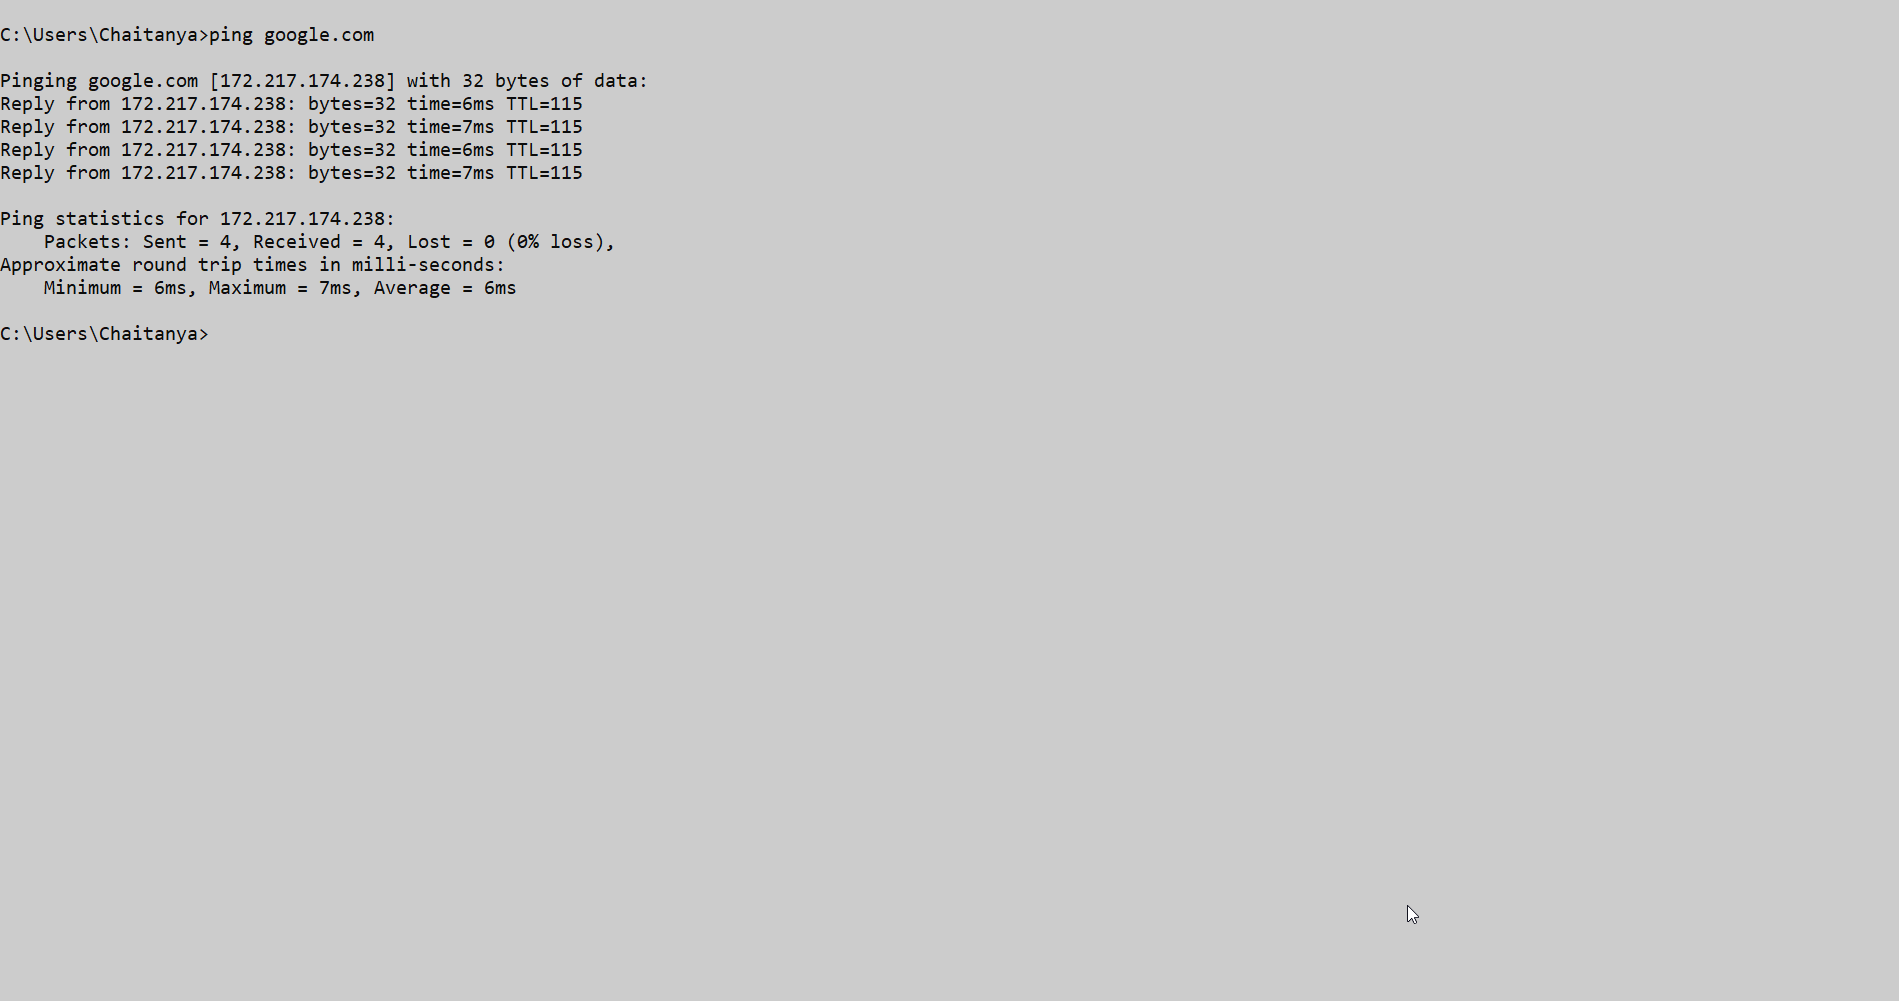
\includegraphics[]{ping.png}
    \caption{Ping Command Output}
    \label{fig:ping_output}
\end{figure}

\clearpage % Ensures the next content starts on a new page

\subsection{\texttt{traceroute}}
The \texttt{traceroute} command traces the path taken by packets from the source machine to a destination host, showing the routers and devices along the way. It helps in diagnosing network routing issues or delays.

\subsubsection{Options}
\begin{itemize}
    \item \texttt{-h \textless max\_hops\textgreater} - Specifies the maximum number of hops (routers) to trace.
    \item \texttt{-w \textless timeout\_seconds\textgreater} - Sets the timeout for waiting for each reply.
    \item \texttt{-m \textless max\_ttl\textgreater} - Specifies the maximum time-to-live (TTL) for the traceroute packets.
    \item \texttt{-n} - Displays IP addresses instead of domain names.
    \item \texttt{-I} - Uses ICMP echo requests instead of UDP packets.
    \item \texttt{-T} - Uses TCP packets instead of UDP packets.
    \item \texttt{-p \textless port\_number\textgreater} - Specifies the destination port for TCP packets.
    \item \texttt{-q \textless queries\_per\_hop\textgreater} - Specifies the number of probe packets sent at each hop.
    \item \texttt{-l \textless packet\_size\textgreater} - Sets the packet size.
\end{itemize}

\subsubsection{Example 1}
To trace the route to a host (e.g., google.com):
\begin{verbatim}
traceroute google.com
\end{verbatim}

% \subsubsection{Command Information and Options}
% Add content here.

\subsubsection{Command Output}
\begin{figure}[htbp]
    \centering
    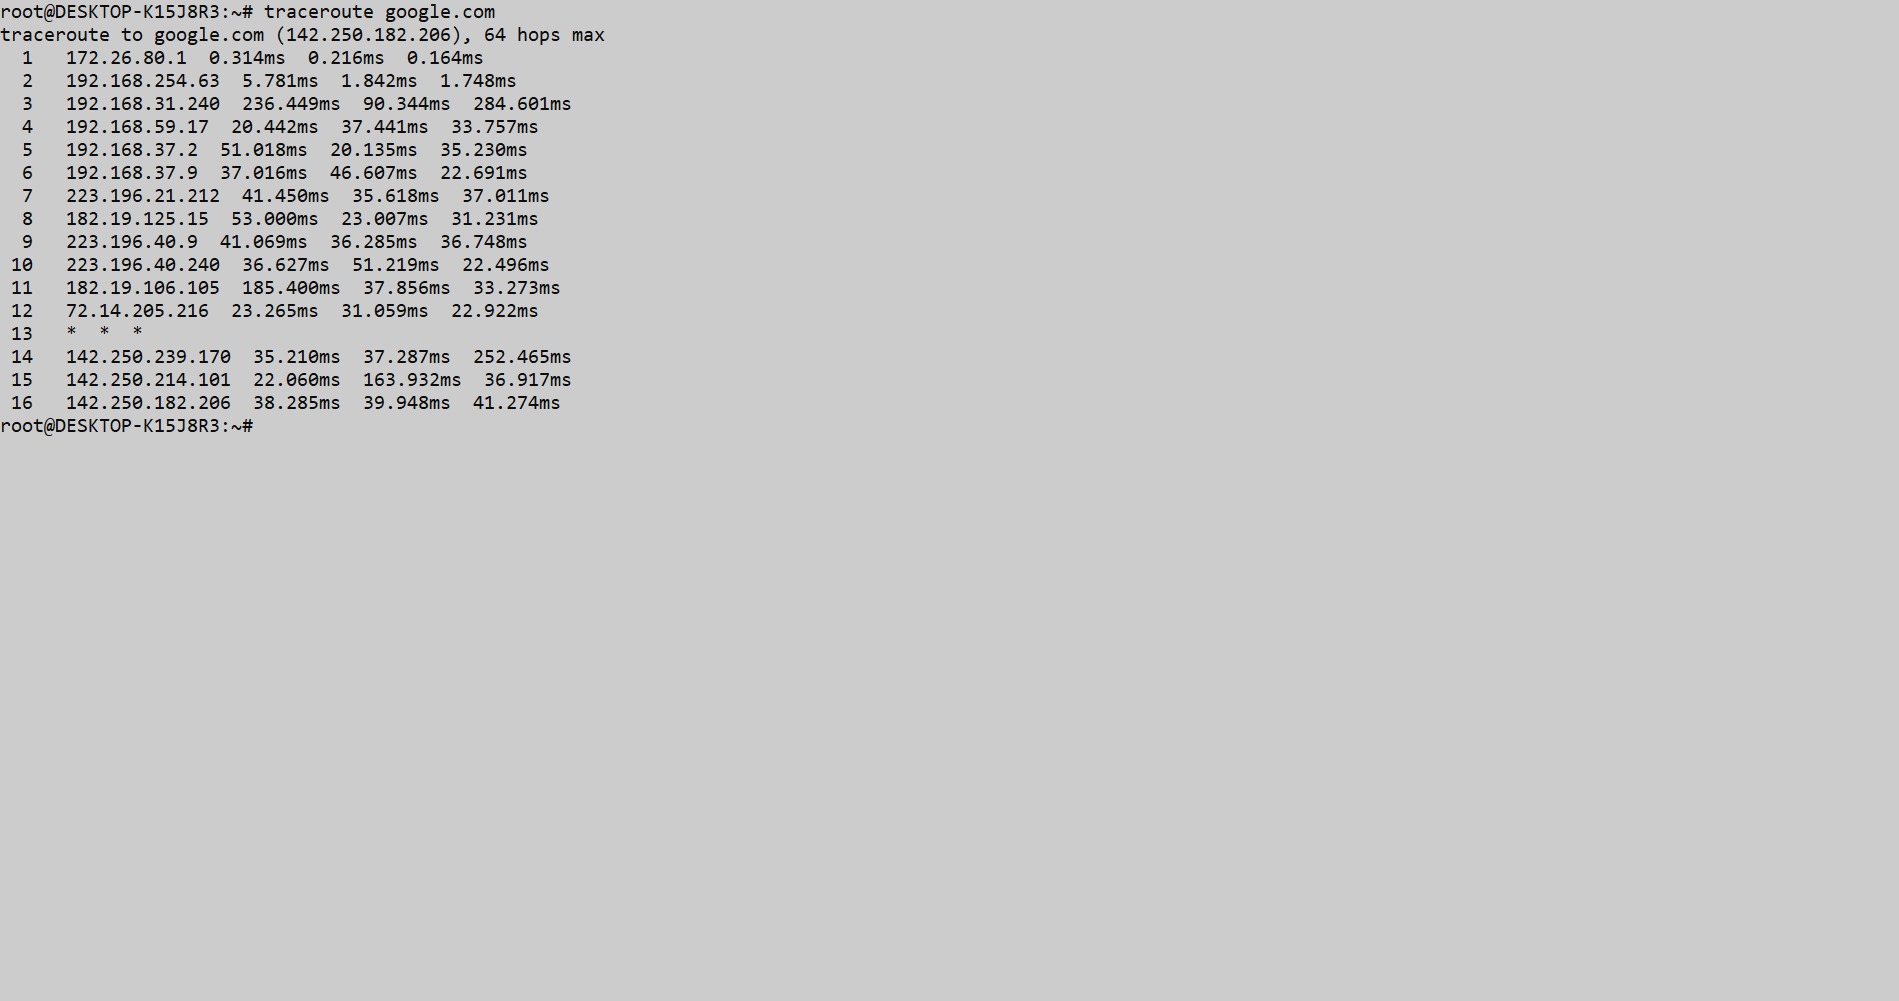
\includegraphics[]{traceroute.png}
    \caption{Traceroute Command Output}
    \label{fig:traceroute_output}
\end{figure}

\clearpage  % Ensures the next content starts on a new page
\subsection{\texttt{nslookup}}
The \texttt{nslookup} command is used to query DNS servers for domain name or IP address information. It is helpful for troubleshooting DNS-related issues.

\subsubsection{Options}
\begin{itemize}
    \item \texttt{-type=\textless record\_type\textgreater} - Specifies the type of DNS record to query (e.g., A, MX, NS).
    \item \texttt{-timeout=\textless seconds\textgreater} - Sets the timeout for a response.
    \item \texttt{-debug} - Enables debug mode for detailed output.
    \item \texttt{-query=\textless domain\textgreater} - Queries a specific domain or IP.
\end{itemize}

\subsubsection{Example 1}
To query the DNS records for a domain:
\begin{verbatim}
nslookup google.com
\end{verbatim}

\subsubsection{Command Output}
\begin{figure}[htbp]
    \centering
    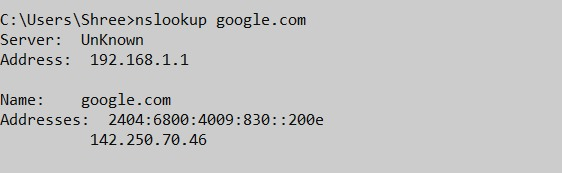
\includegraphics[]{nslookup.png}
    \caption{NSLookup Command Output}
    \label{fig:nslookup_output}
\end{figure}
\clearpage  % Ensures the next content starts on a new page
\subsection{\texttt{pathping}}
The \texttt{pathping} command provides detailed information about packet loss and latency along a network route. It combines the features of \texttt{ping} and \texttt{traceroute}.

\subsubsection{Options}
\begin{itemize}
    \item \texttt{/q} - Sets the number of query packets per hop.
    \item \texttt{/n} - Prevents the resolution of hostnames to IP addresses.
    \item \texttt{/h \textless max\_hops\textgreater} - Specifies the maximum number of hops.
    \item \texttt{/w \textless timeout\textgreater} - Sets the wait time for each reply.
\end{itemize}

\subsubsection{Example 1}
To analyze a route with pathping:
\begin{verbatim}
pathping google.com
\end{verbatim}

\subsection{Command Output}
\begin{figure}[htbp]
    \centering
    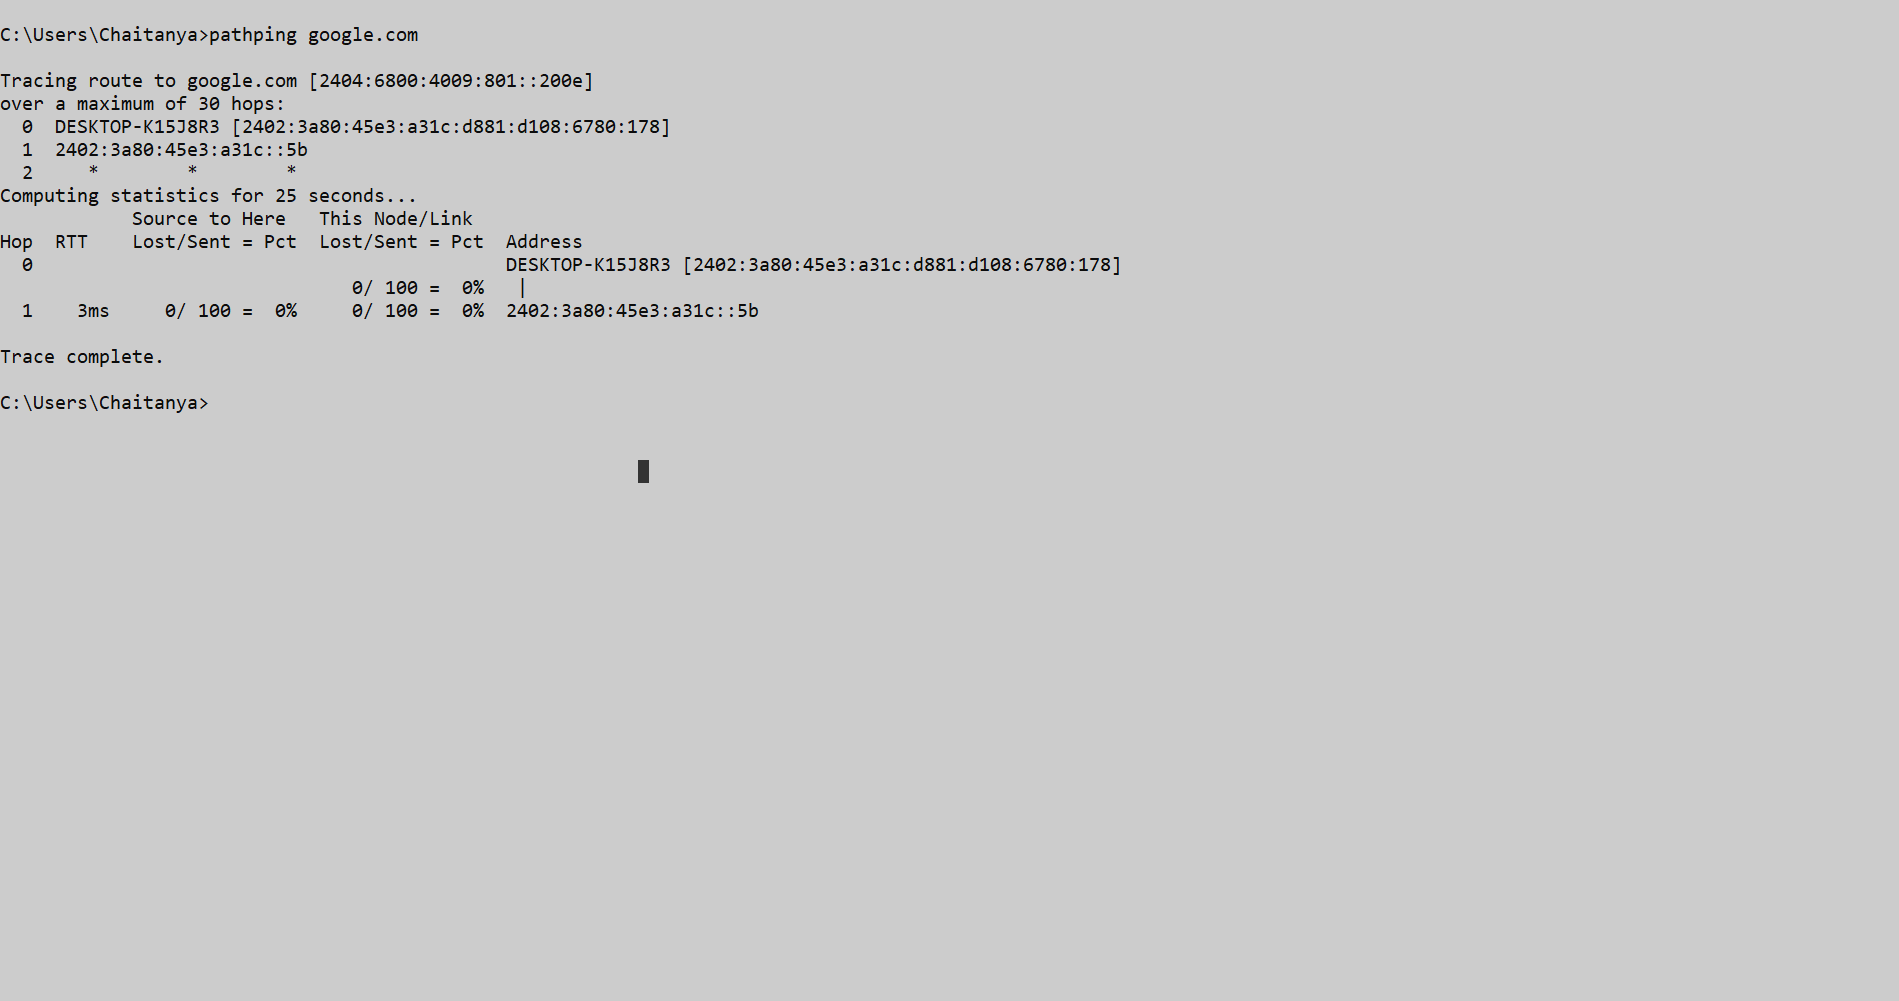
\includegraphics[]{pathping.png}
    \caption{Pathping Command Output}
    \label{fig:pathping_output}
\end{figure}
\clearpage  % Ensures the next content starts on a new page
\subsection{\texttt{tracert}}
The \texttt{tracert} command traces the route packets take to reach a destination. It is primarily used for diagnosing routing issues.

\subsubsection{Options}
\begin{itemize}
    \item \texttt{/h \textless max\_hops\textgreater} - Specifies the maximum number of hops.
    \item \texttt{/d} - Prevents the resolution of IP addresses to hostnames.
    \item \texttt{/w \textless timeout\textgreater} - Sets the timeout for each reply.
\end{itemize}

\subsubsection{Example 1}
To trace the route to a domain:
\begin{verbatim}
tracert google.com
\end{verbatim}

\subsection{Command Output}
\begin{figure}[htbp]
    \centering
    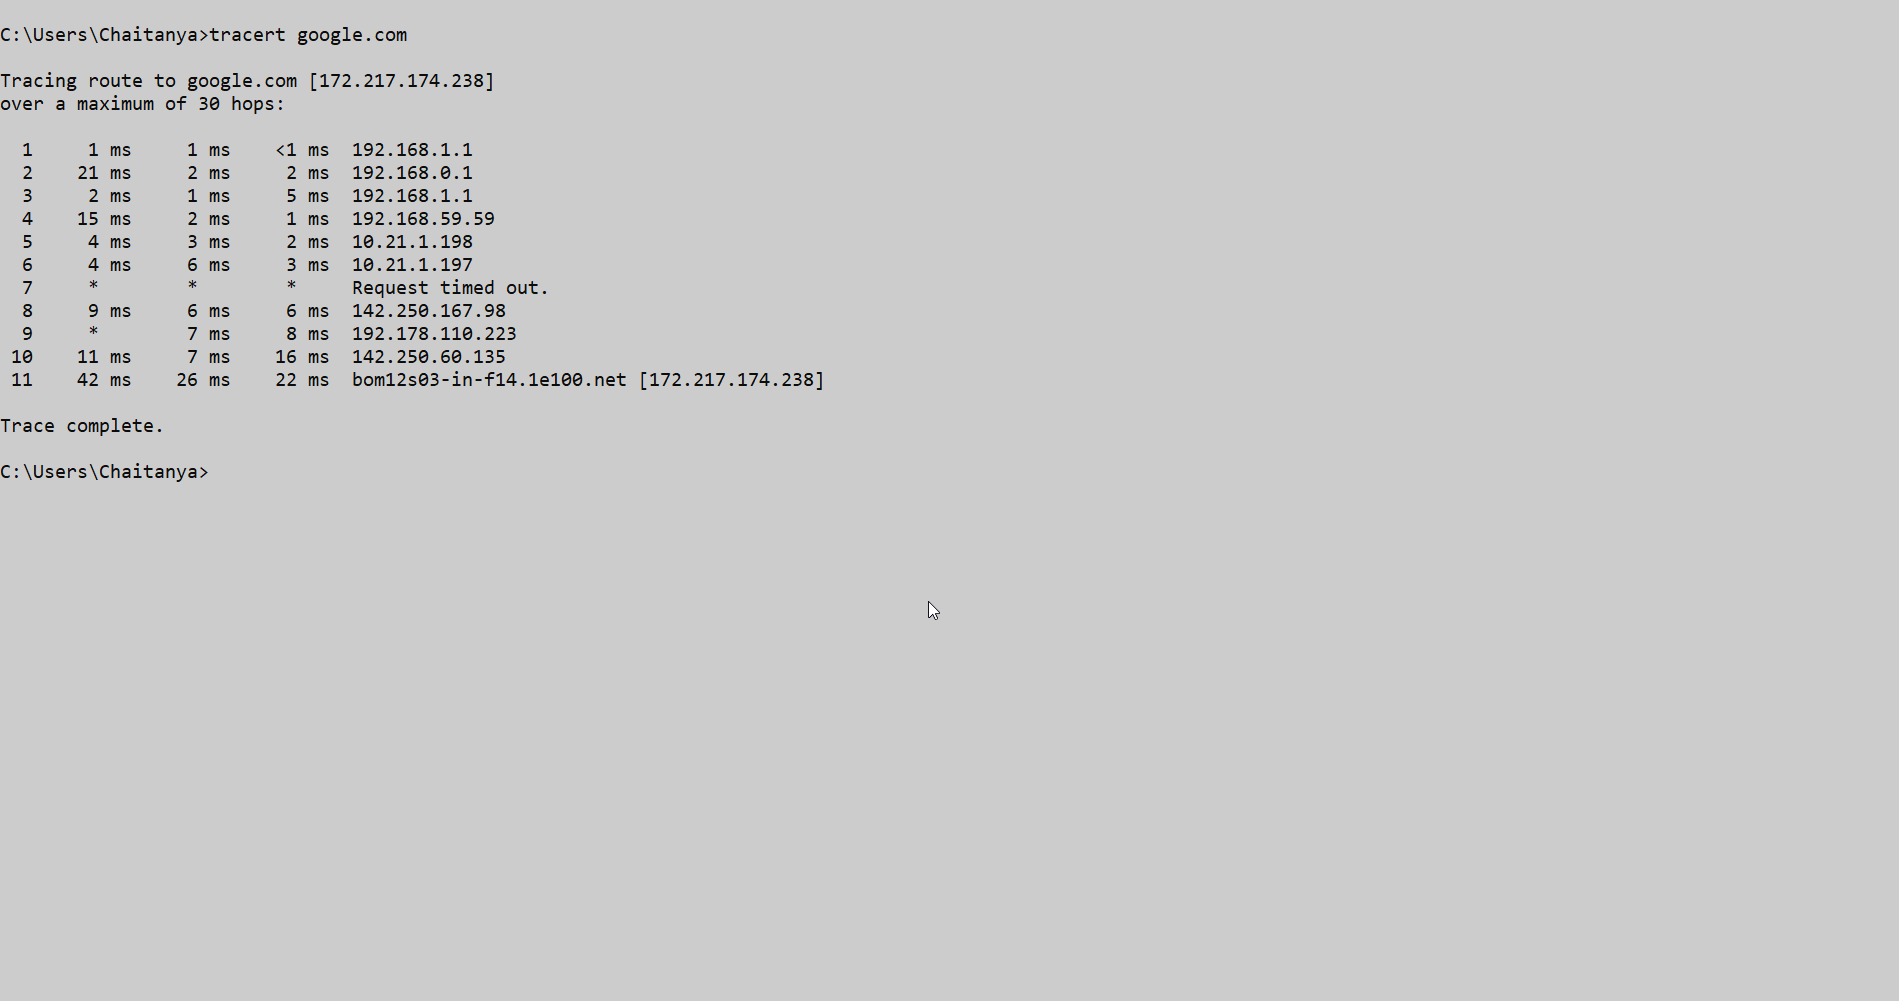
\includegraphics[]{traceroute_output.png}
    \caption{Tracert Command Output}
    \label{fig:tracert_output}
\end{figure}
\clearpage  % Ensures the next content starts on a new page
\subsection{\texttt{netstat}}
The \texttt{netstat} command provides information about active network connections, routing tables, and network statistics.

\subsubsection{Options}
\begin{itemize}
    \item \texttt{-a} - Displays all active connections and listening ports.
    \item \texttt{-n} - Shows addresses and port numbers in numerical format.
    \item \texttt{-r} - Displays the routing table.
    \item \texttt{-s} - Displays statistics for each protocol.
\end{itemize}

\subsubsection{Example 1}
To view all active connections:
\begin{verbatim}
netstat -a
\end{verbatim}

\subsection{Command Output}
\begin{figure}[htbp]
    \centering
    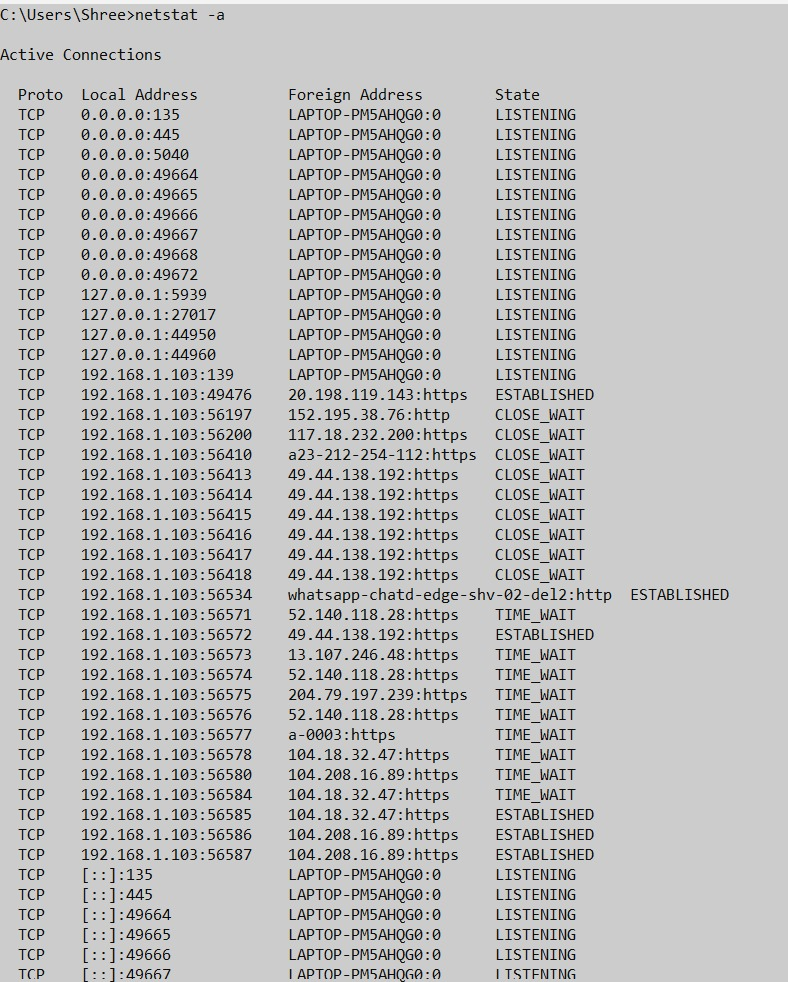
\includegraphics[]{netstat-aCom.jpeg}
    \caption{Netstat Command Output}
    \label{fig:netstat_output}
\end{figure}
\clearpage  % Ensures the next content starts on a new page
\subsection{\texttt{arp}}
The \texttt{arp} command manages the ARP cache, resolving IP addresses to MAC addresses.

\subsubsection{Options}
\begin{itemize}
    \item \texttt{-a} - Displays all entries in the ARP cache.
    \item \texttt{-d \textless ip\_address\textgreater} - Deletes a specific entry.
    \item \texttt{-s \textless ip\_address\textgreater \textless mac\_address\textgreater} - Adds a static ARP entry.
\end{itemize}

\subsubsection{Example 1}
To view the ARP cache:
\begin{verbatim}
arp -a
\end{verbatim}

\subsection{Command Output}
\begin{figure}[htbp]
    \centering
    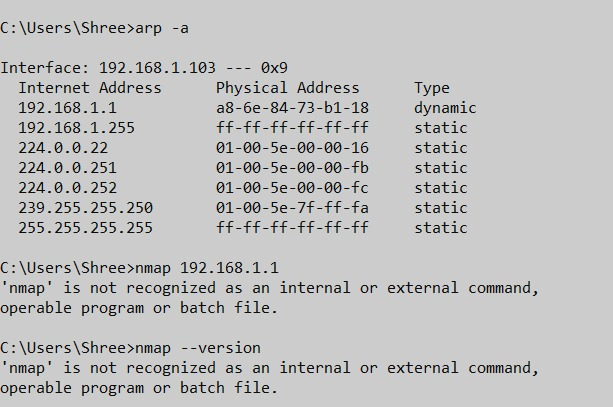
\includegraphics[]{arp.jpg}
    \caption{ARP Command Output}
    \label{fig:arp_output}
\end{figure}
\clearpage  % Ensures the next content starts on a new page
\subsection{\texttt{nmap}}
The \texttt{nmap} command scans networks to discover hosts, services, and open ports.

\subsubsection{Options}
\begin{itemize}
    \item \texttt{-sP} - Performs a ping scan to identify live hosts.
    \item \texttt{-sT} - Performs a TCP connect scan.
    \item \texttt{-p \textless port\_range\textgreater} - Scans specified ports or ranges.
    \item \texttt{-A} - Enables advanced options like OS detection and version scanning.
    \item \texttt{-v} - Displays verbose output.
\end{itemize}

\subsubsection{Example 1}
To scan for open ports on a host:
\begin{verbatim}
nmap -sT google.com
\end{verbatim}

\subsection{Command Output}
\begin{figure}[htbp]
    \centering
    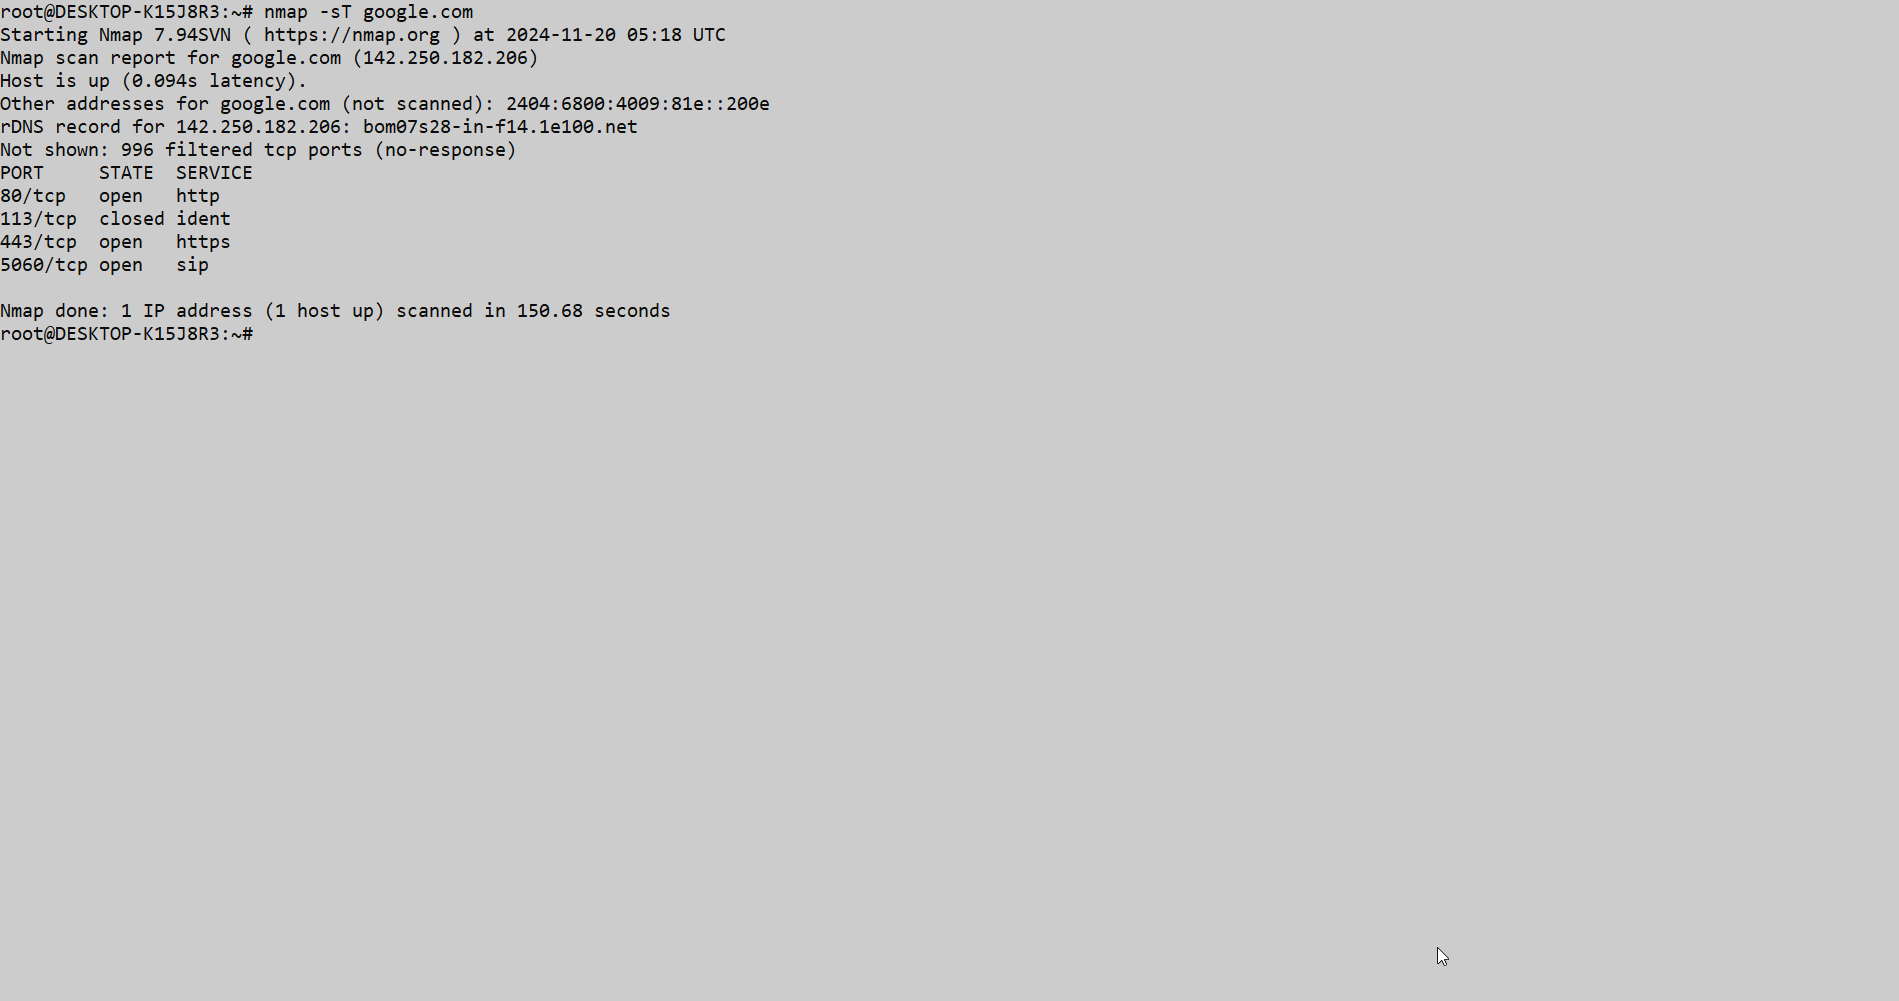
\includegraphics[]{nmap.png}
    \caption{Nmap Command Output}
    \label{fig:nmap_output}
\end{figure}
\clearpage  % Ensures the next content starts on a new page
\end{document}


